Ben Trout

2015-01-09

Building

\begin{tabular}{|p{4cm}|p{8cm}|}
\hline
Telescoping tube&
The tube has two sections each made of wood and both the same height. The smaller section is attached to the robot via two of the smallest one hole channels at the base of the small section. The small section is grounded to the robot at about 3 inches from the floor as to make sure it doesn’t catch the robot. The larger section slides over the smaller section with two slots cut out of the base to fit over the two channels supporting the smaller section. The Larger section is secured to the top most slide of our linear track. 
\\
\hline
Linear drawer slide track&
As a group we decided the best way to extend our tube from a compiled position would be to attach it directly down the middle of our robot connected to the center beams that form the back bars of our robot. Filip attached the two L brackets that are screwed to the back beams of our robot and figured out the best place to fix the slides. The track is two linear drawer slides bolted to each other. Me and Nick drilled out the corners of the biggest tracks of each linear slide. We then stuck bolts through the holes with a spacer on each bolt. With the help of Alex we were able to route the string starting from a motor, up to the top of the first track down to the bottom of the first track, up to the top of the second track and tied to the section bolted to the slides. This would create a pulley system that would allow a motor to easily lift up linear drawer slides to any desired height whether that be 30, 60, or 90cm. 
\\
\hline
Ramp and guides&
The ramp is essentially one square piece of polycarb that Nick and Alex bent using a heat gun to get the right shape of the curve. I cut out two guides out of the polycarb and taped those to the inside of the smaller section of the tube. We made sure the larger section could still slide over the smaller section of the tube. The guides have overhangs that filip helped me drill out and attach to the robot with bolts.
\\
\hline
Deflector&
Matt originally designed the deflector and his design idea is what we ended up going with. It is pretty simple: It has two forty five degree angles with a flat section between the two angles. The ball comes up gets deflected of one of the other and through a small hole into the tube. Matt’s design had a couple flaws and Alex was able to redesign it perfectly centering the exit of the deflector around the hole of the tube we are dragging around. 
\\
\hline
\end{tabular}

\section*{Telescoping tube}
The tube was initially made into three pieces that fit inside each other. It was relatively easy to make each different section as it took some quick measuring. Each smaller section was exactly two width of the wood smaller than the section before. It wasn’t until we had attached the linear drawer slides that we really figured out how to assemble the tube. How we made sections of the tube we decided it wasn’t feasible to use all three sections. Instead we used two, the smallest and biggest. One of our biggest fears was that by going biggest to smallest would leave edges the balls could catch on their way up and fall back down. But we needed a way to secure the inmost box to robot and this isn’t possible to do with the smaller box if the larger one needs to slide over it. But we came up with a solution. I cut out slots in the large box while Nick attached two single channel pieces to the base of our robot. Nick had to make sure to put spacers between the channel and back bar so that as the sections came back down they didn’t catch on the bolts securing everything. The small section is bolted to these channels and the big box is still able to slide over because of the slots cut into it. The only problem left with this mechanism is it leaves a big gap for balls go go flying out. Our plan now is to attach some sort of cloth that is rolled up at the bottom of the large section of the tube and as it is raised the cloth will fall down and block balls from flying across the room. By using cloth we can bunch it up and allow for us to still be inside the 18in by 18in starting position. 

\section*{drawer slides}
I went on the Lowes sight and figured out what side drawer slides we could get and still be in the 18in box. I ended up choosing the 16in drawer slides from Lowes. Me and Nick were put in charge of putting all the slides together and making a pulley system that would lift the tube. Initially we had attached the two slides to each other from small end to small end. We drilled out holes in the large sections of the slides, one at the top and one at the bottom. Me and Nick then made a pulley system that had string threaded through spacers that were bolted to the slides. The problem with mine and Nicks design was that we could only lift the slides to the 60cm goal as our pulley wasn’t set up right. With the help of Alex on a later day we were able to make the correct pulley pattern that allows us to get to the 120cm goal. All me and Nick really had to do was switch the slides so they were attached small section of first to big of second, and then we tied the string of to the top section of our tube instead of the bottom final loop of the pulley. We had our biggest difficulties with determining in drilling and placement of the slides. In drilling we had to be very precise and the fact that the slides have rounded edges made it very hard not to slip, in the future it would be helpful to have a center punch. Placement was another big decision. As a group we decided that the middle of the back beam would be ideal, but this would push our ramp up, which would force us to move our spinner up, which would force us to cut our intake down, and this just wasn’t feasible as it wouldn’t be able to intake the small balls anymore. Filip and Matt were then put in charge of taking out the back channels of our robot and replacing them with angled bars would be the best option. This would allow us to move the whole assemble back to its original position and we wouldn’t have to cut anything down. 

\section*{create guides and ramp}
I was put in charge of creating the ramp and guides with the help of David and another team member from FRC. We used the drawing tool in creo that makes a drawing of one side of a model and can print that out on paper. We cut out this drawing and traced two of them on polycarb sheet. Using a ban saw we cut out both side panels of the ramp. Using the measure tool in creo I was able to figure out the dimension of our ramp and back base. Using a heat gun we were able to bend the back piece and braces of the guides that get bolted to the robot. Bending was pretty difficult and by no means reliable. The back piece was so bent well and when we put the ramps into the bends of the back piece to attach them the guides didn’t even touch the ends of the back piece as the bends weren’t perfect 90s. We tried epoxy first, but the surfaces didn’t meet enough for this to be effective. We ended up drilling holes in the corners of the bends and bolting the ramp to the guides. This ended up not being a good idea at all because the bolts would get in the way of the ramp. Once we had the tube attached to the robot though it became a lot more clear how we could attach the guides and ramp. The guides could be taken of our poorly created back piece and merely tapped to the sides of the small section of the tube. Our initial idea for creating the ramp was to bend it around a piece of wood that has a 6in radius to get a perfect curve. We didn’t have time to do this and Alex and Nick just had to bend it one piece at a time. For the next tournament we will definitely remake the ramp.

\section*{Deflector}
Matt was initially in charge of the deflector and his design is what we ended up going with. It was pretty simple, but because we moved our tube around from where we initially thought it would go the deflector had to be remade. Alex used a bunch of measurements and designing to create a deflector that is directly over the tube. One of the biggest problems was having the deflector start inside the 18in by 18in. Nick came up with the idea of putting rubber bands to the inside of the deflector and looping them around the top part of linear slides. The deflector is laid at a 180 degree angle to the the outer tube in the starter position. At the beginning the spinner spins around and whacks the deflector that raises up. Once the deflector is above a 90 degree angle the rubber bands take it the rest of the way and flip it into position. 

\begin{center}
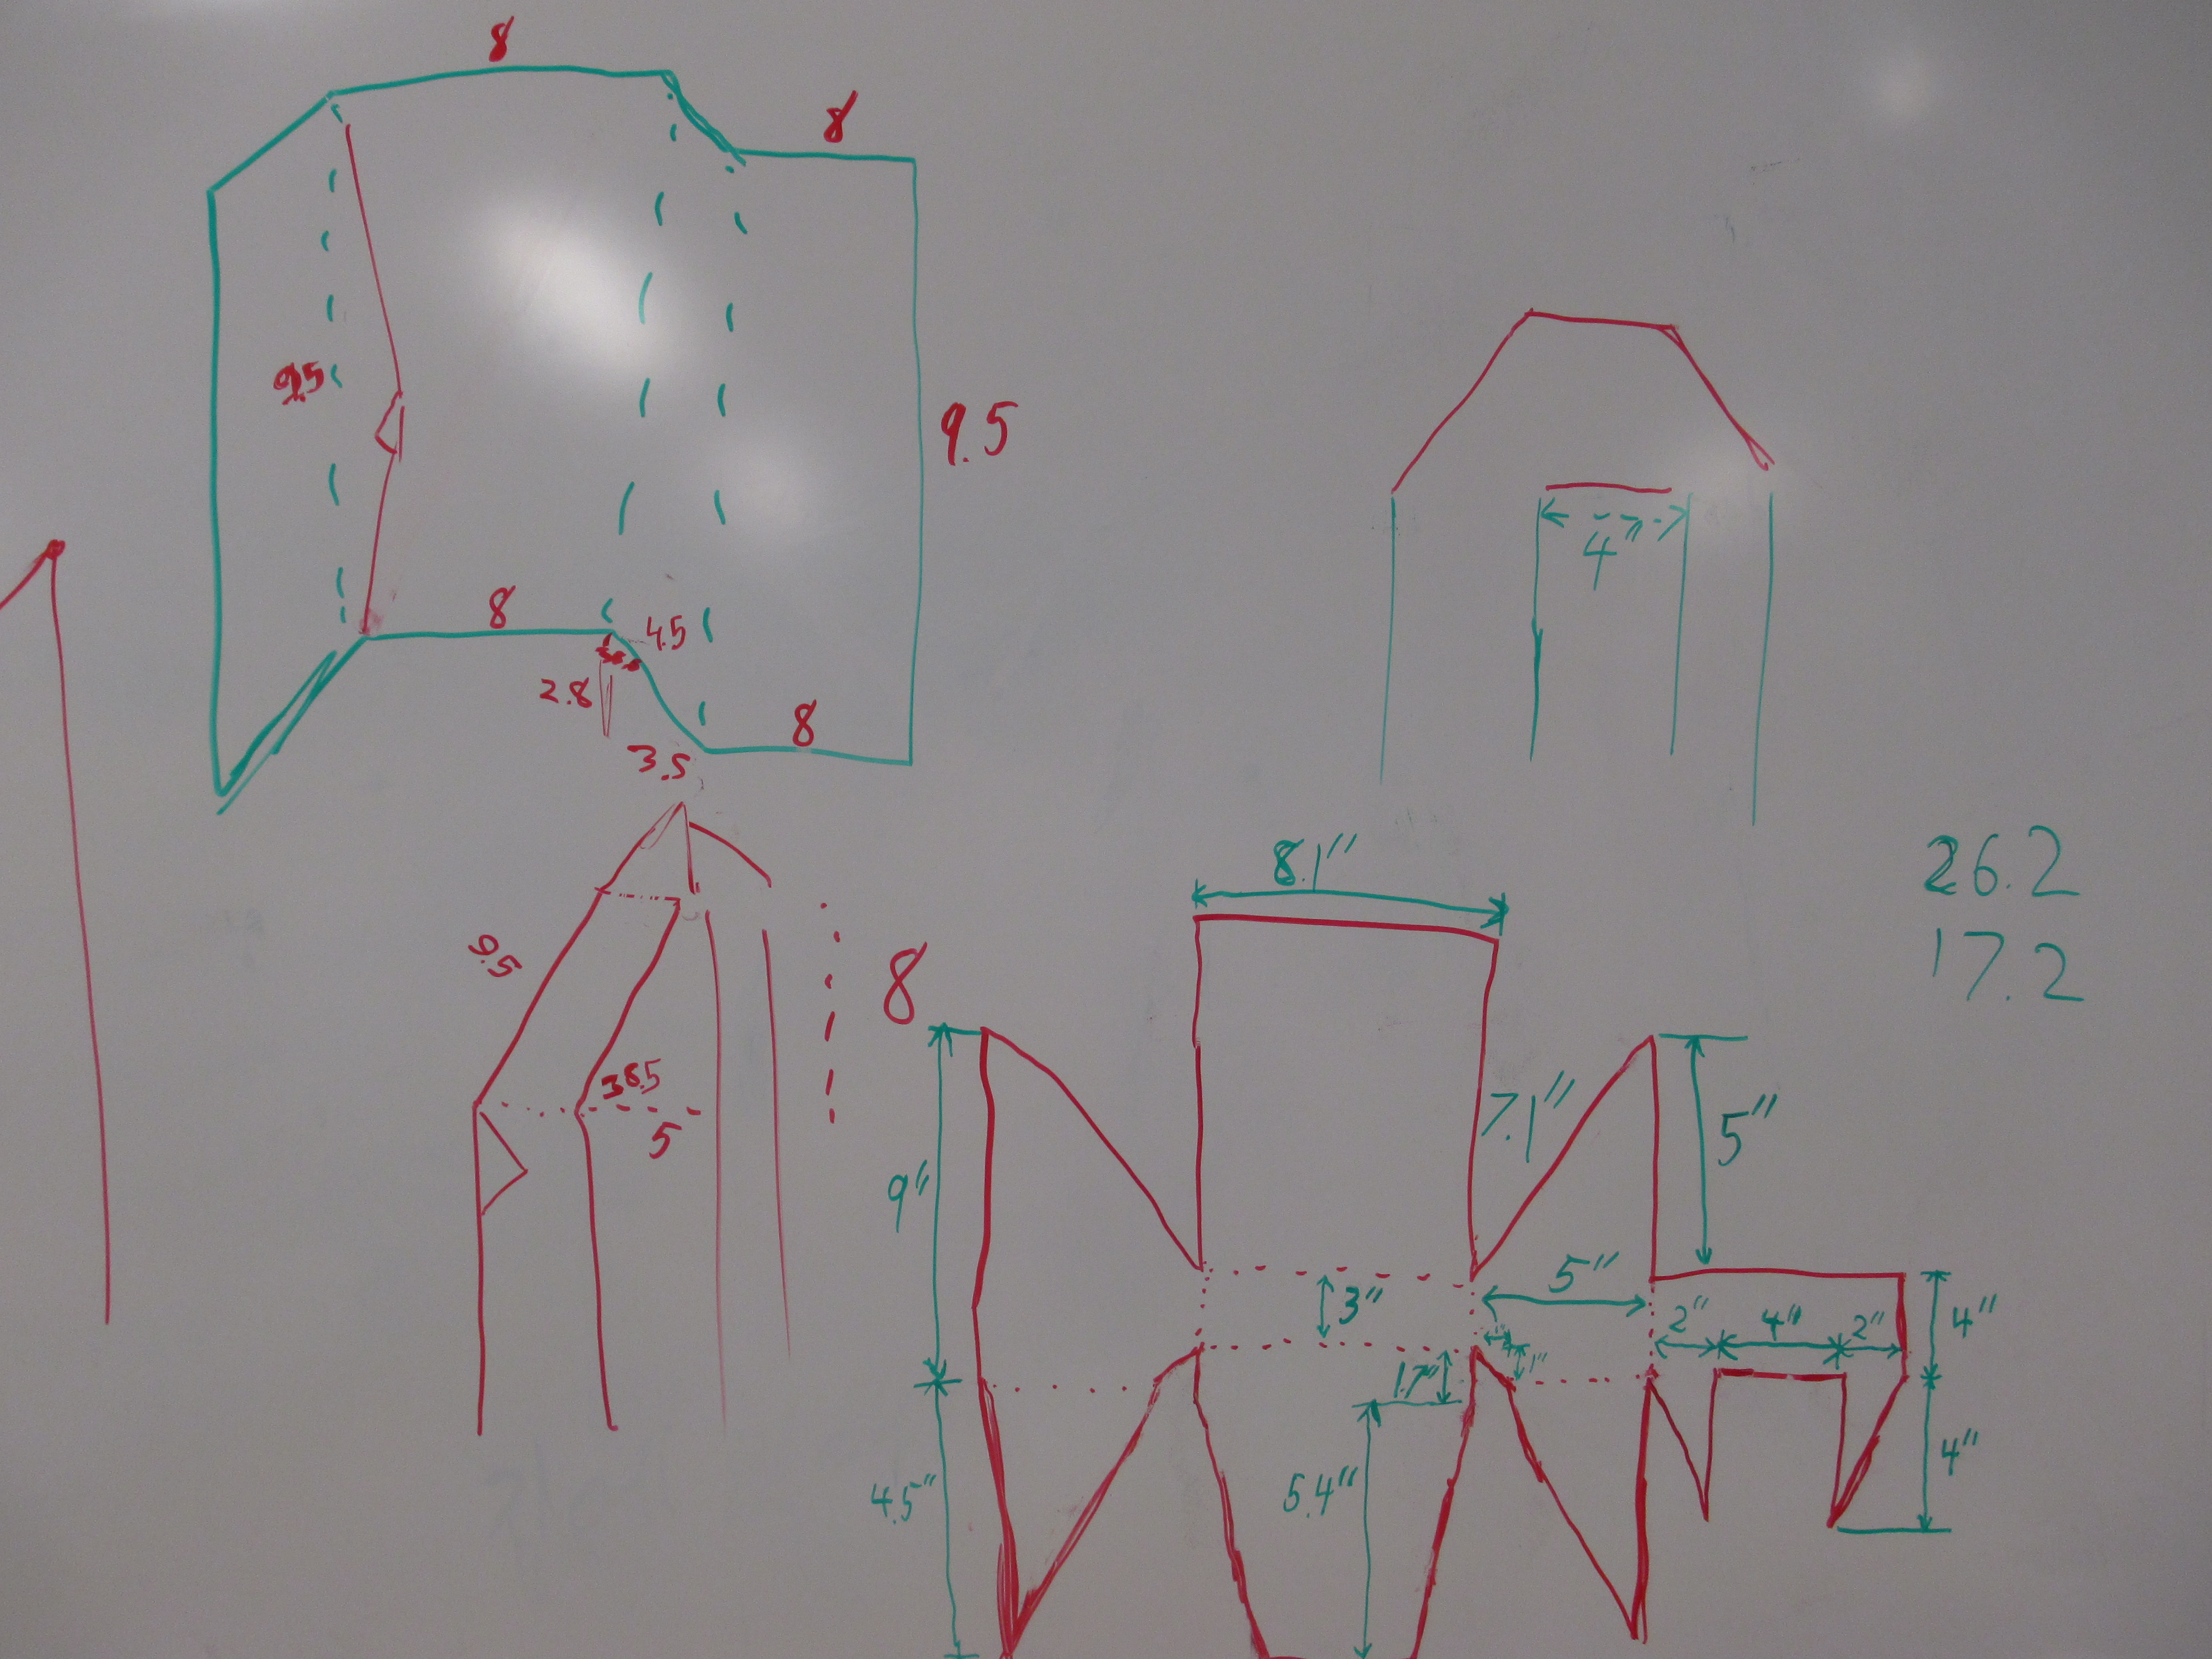
\includegraphics[width=10cm]{./Entries/Images/DeflectorDrawing.jpg}
\end{center}

Alex’s calculations of the deflector

\begin{center}
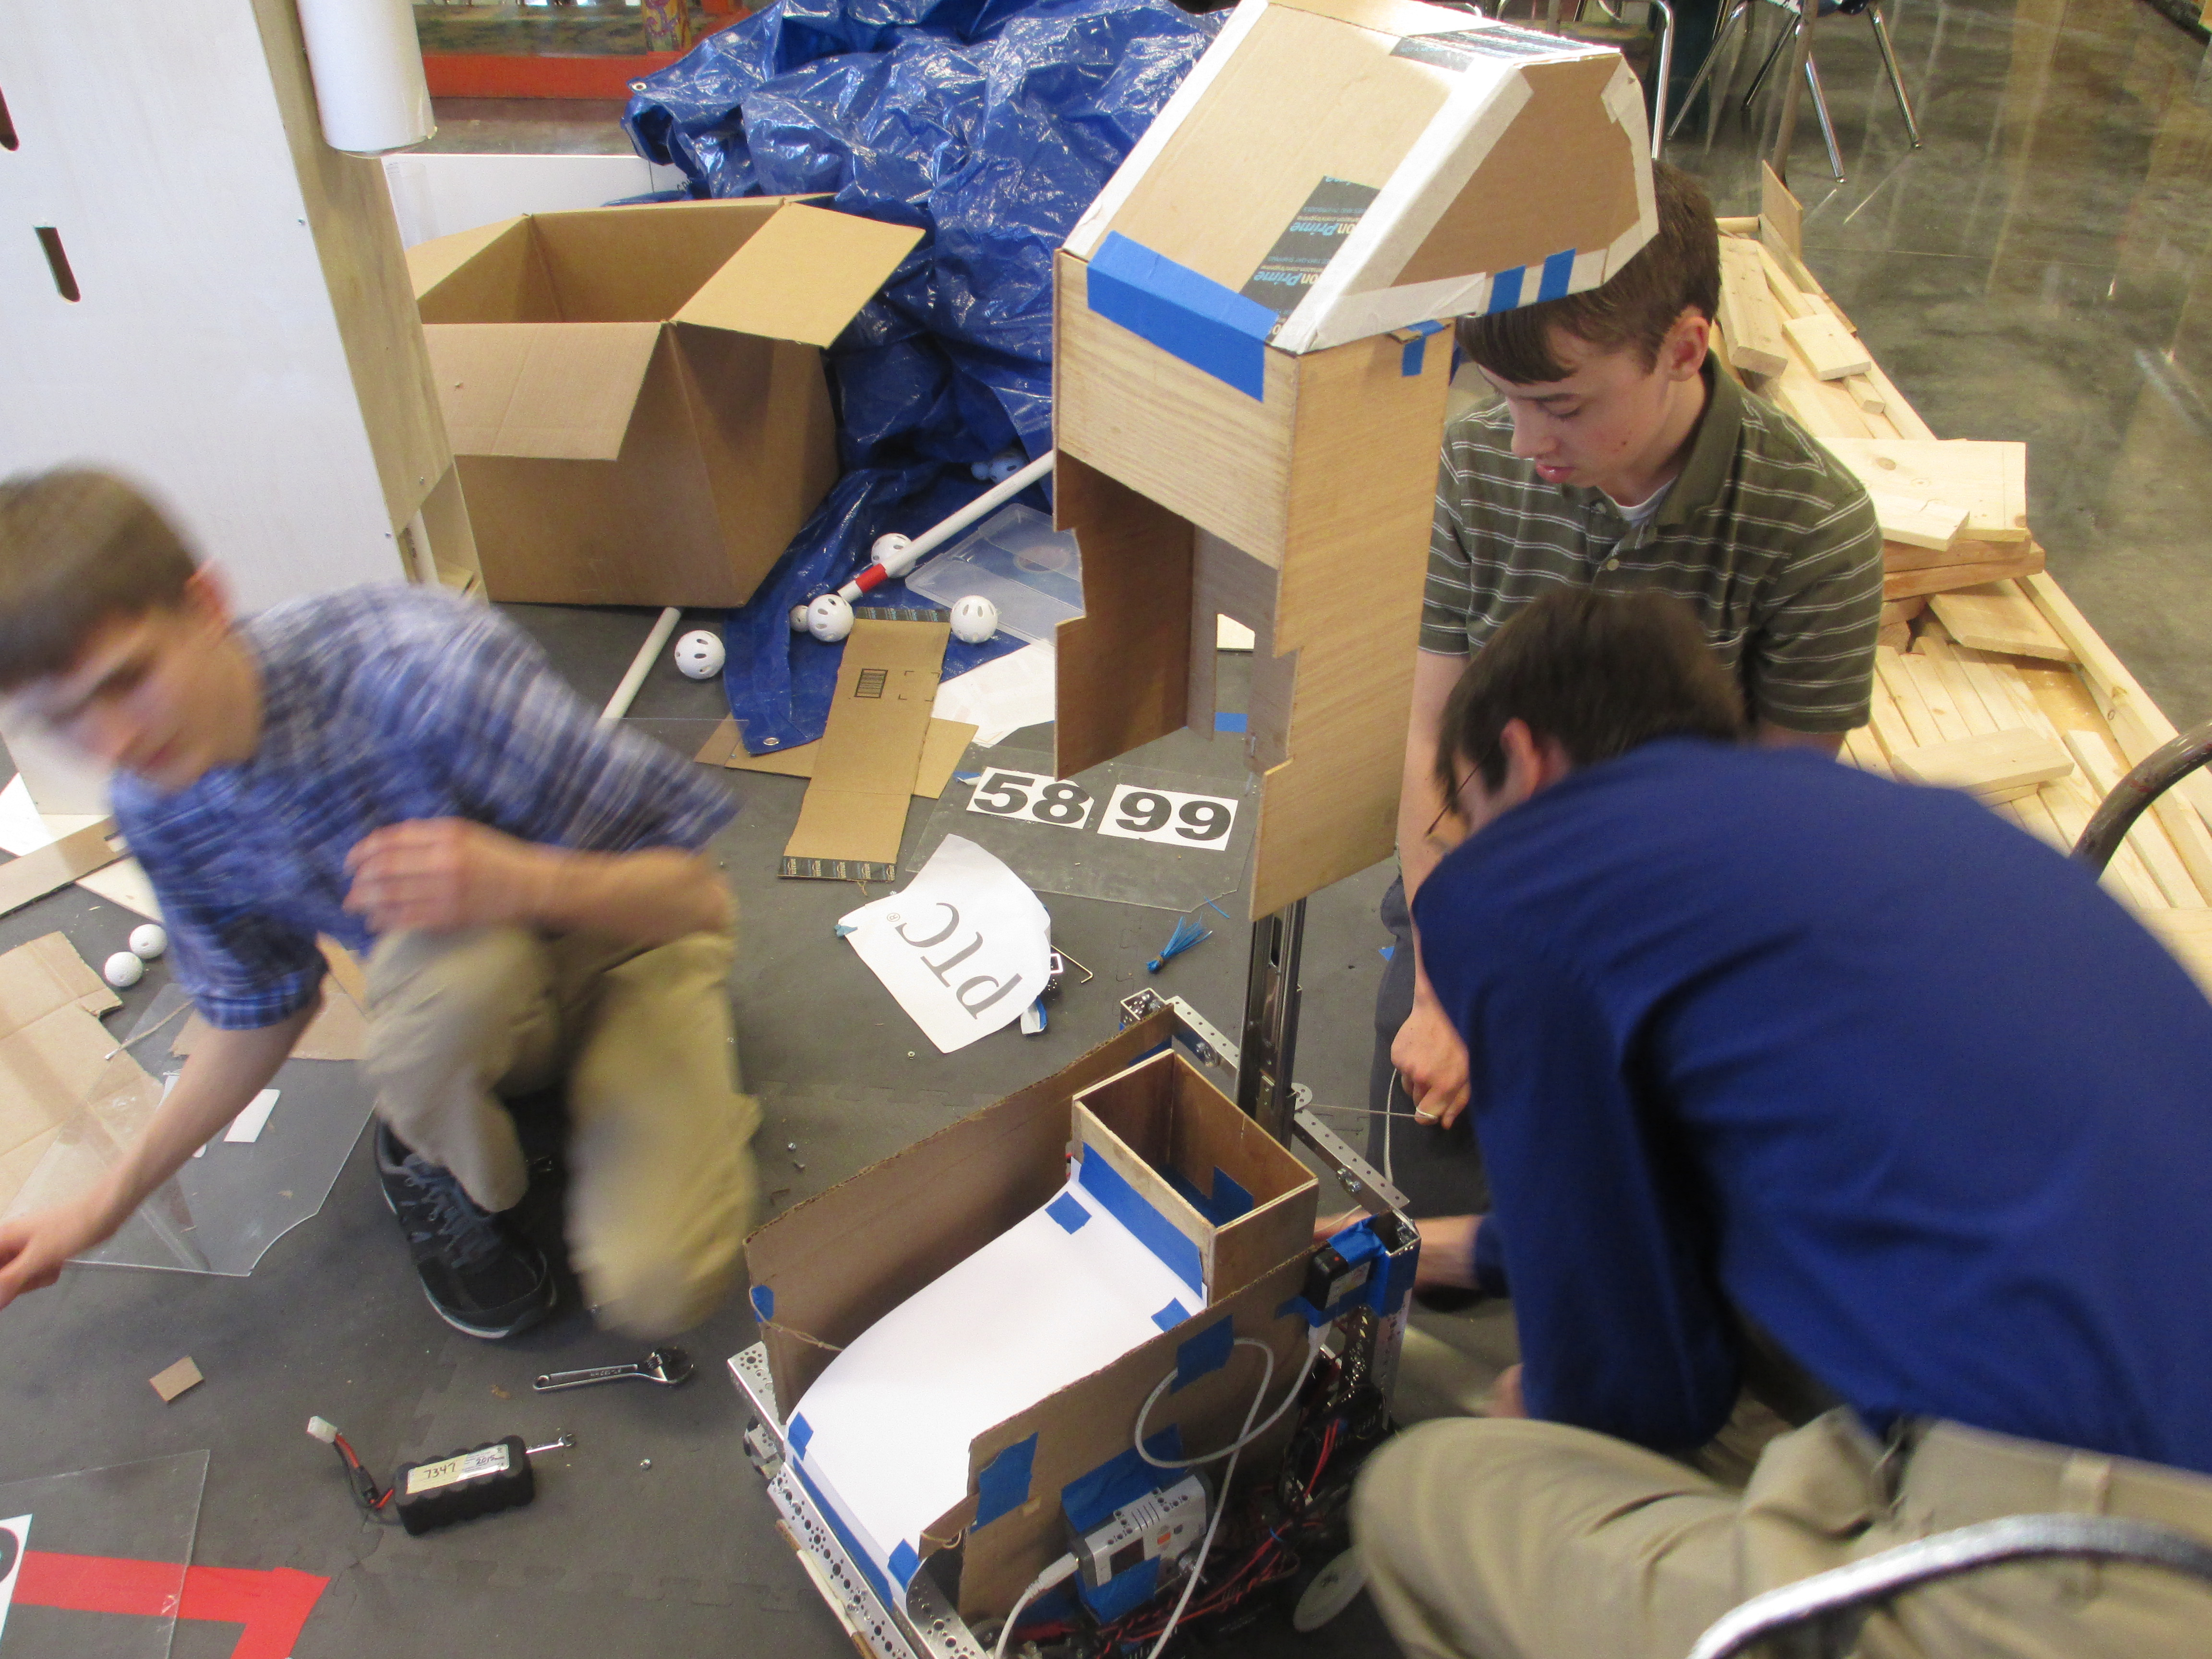
\includegraphics[width=10cm]{./Entries/Images/SlideUP.jpg}
\end{center}

Linear slide and box tube in up position. Deflector flipped up.

\begin{center}
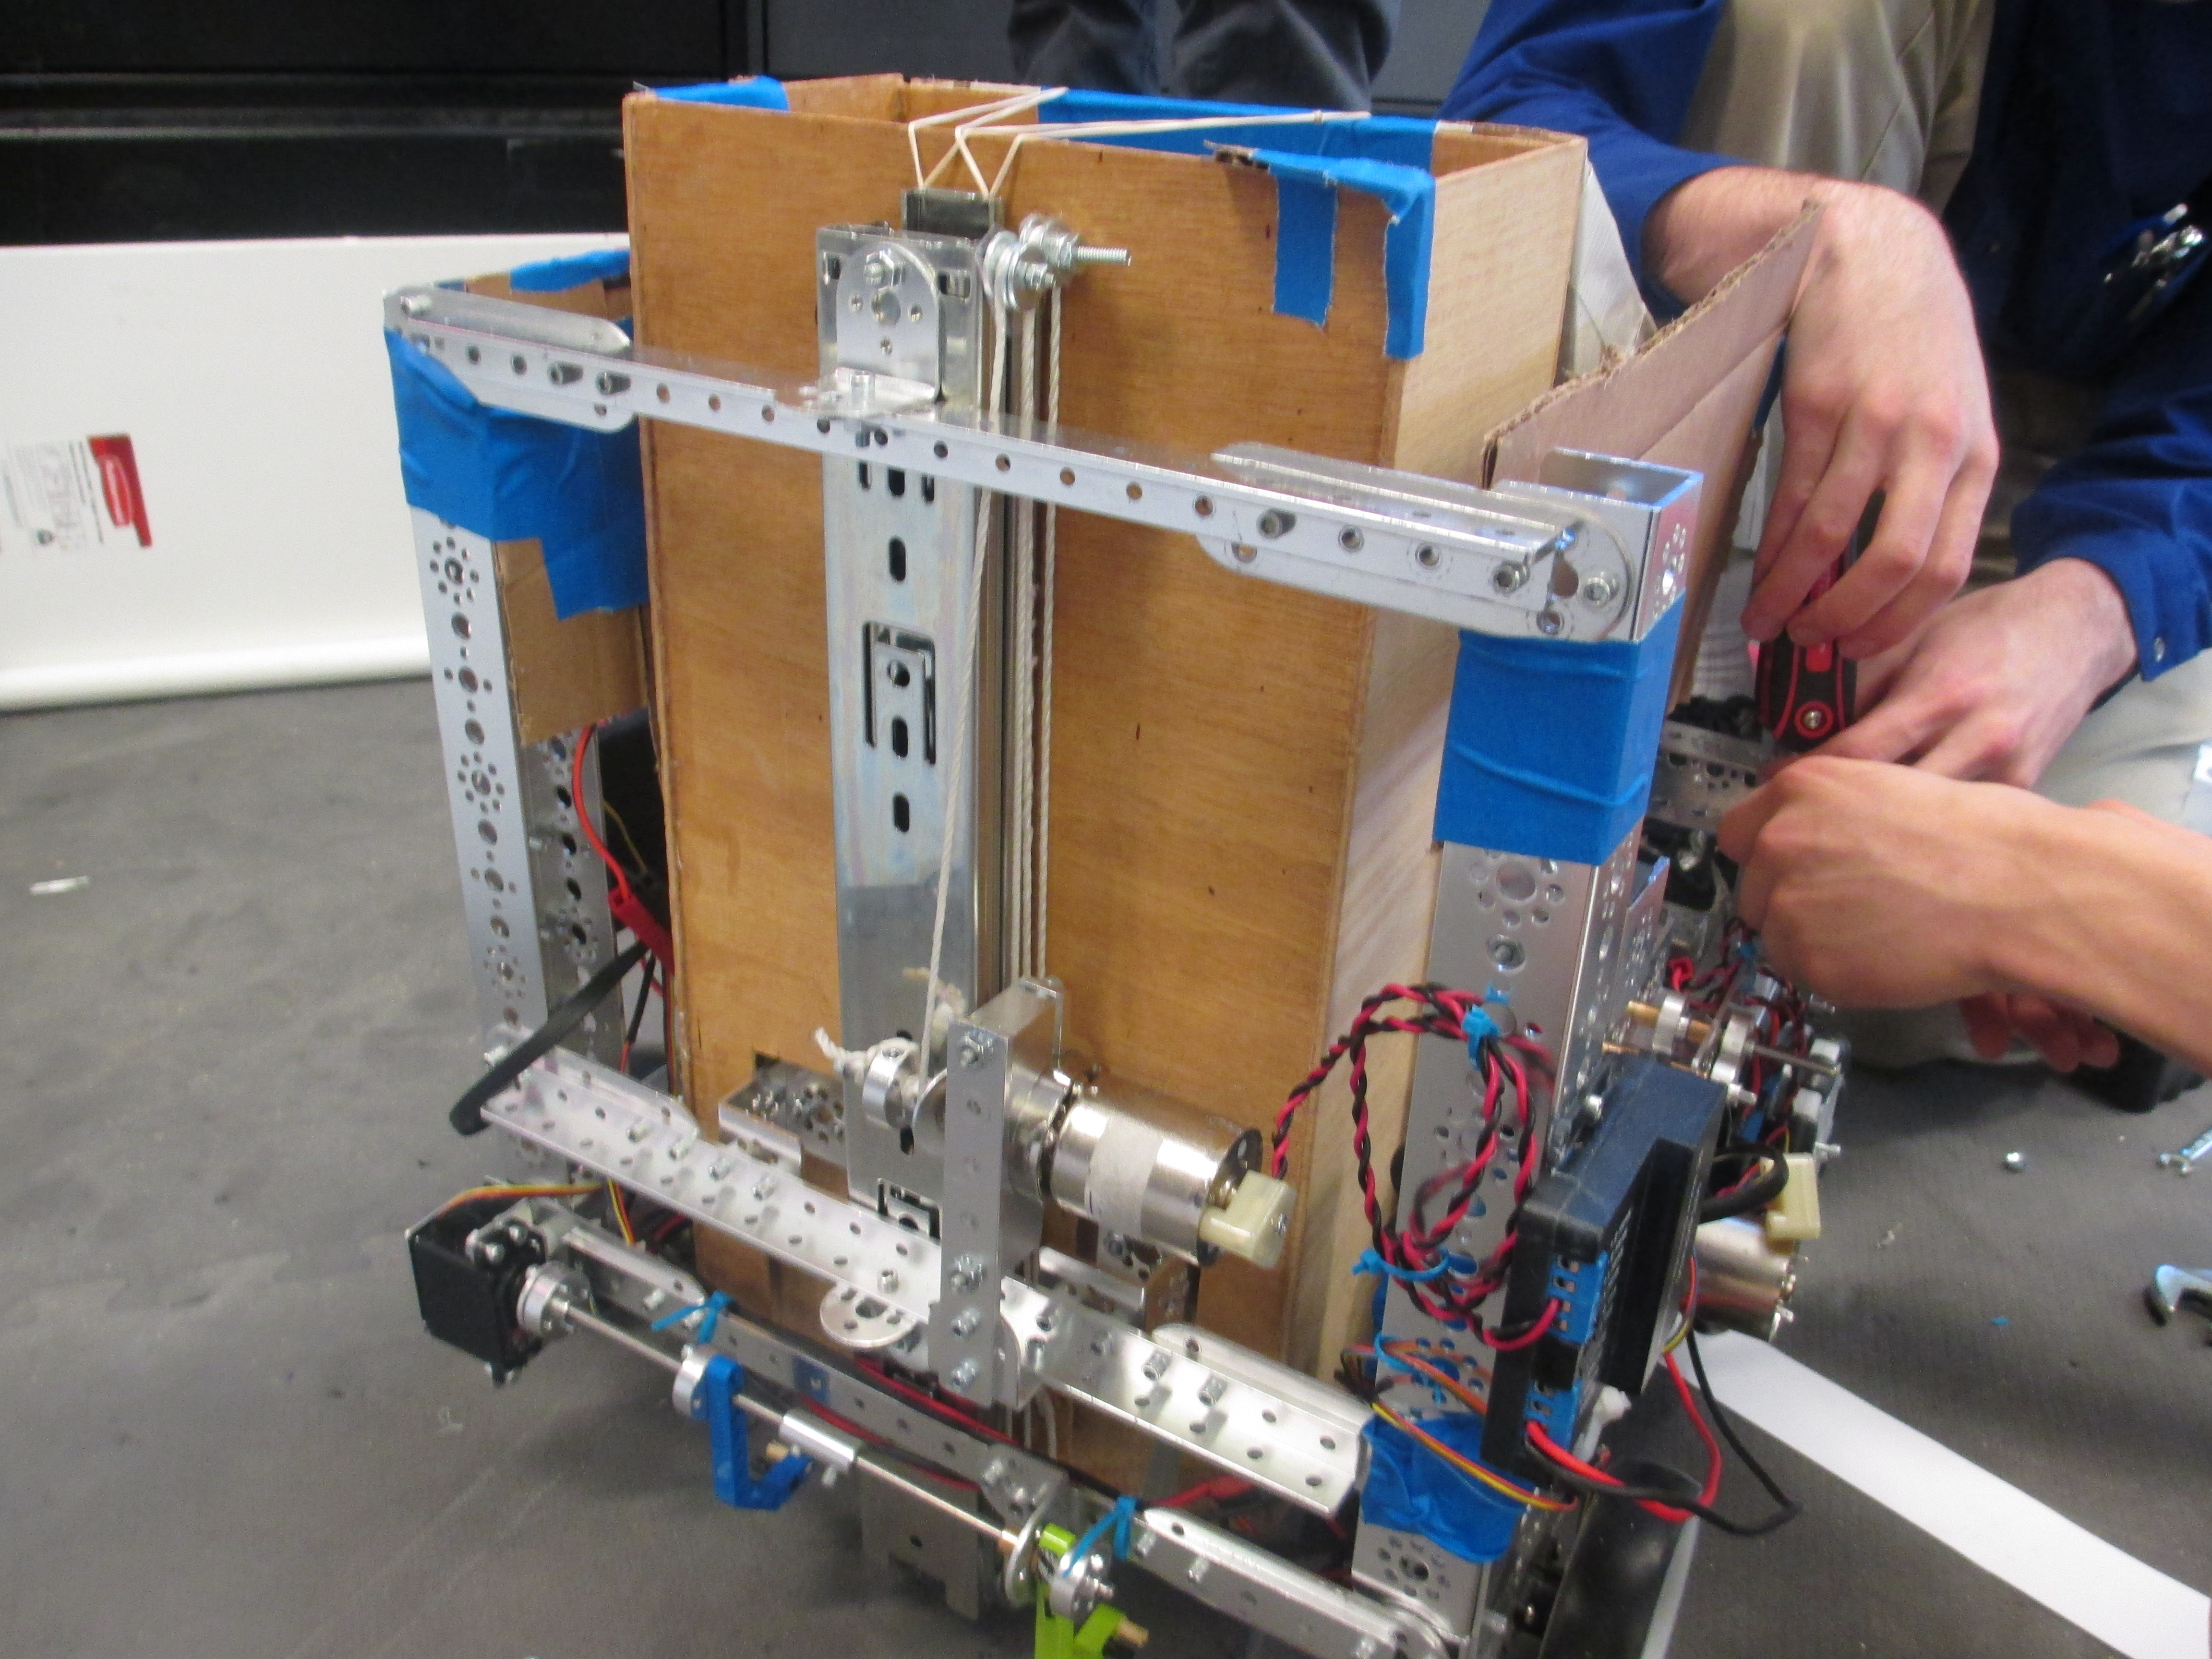
\includegraphics[width=10cm]{./Entries/Images/SlideDown.jpg}
\end{center}

Linear slide and pulley in down position.

\section*{getting ready for competition}
Our whole team has been getting ready for competition making sure the robot is competition worthy, but David has been mainly in charge of this. He has gone through all the specifications of our robot making sure it is not illegal in any form and has all the necessary parts. The rest of us have mainly working on making sure the robot starts in the 18in by 18in box and other small tasks.